\section{Implementation and Deployment}
\label{sec:cfa:impl}

This section presents our implementation of \dda 
 and highlights engineering solutions to address practical challenges 
 in operational settings (e.g., avoiding bulk data loading and 
speeding up development iterations).

\subsection{Implementation of \dda Workflow}
\label{subsec:cfa:impl:workflow}

%Recall that \dda logically consists of three stages 
%running at different timescales (\Section\ref{subsec:scalability}). 
\dda's three stages are implemented in two different locations:
a centralized backend cluster and geographically 
distributed frontend clusters as depicted in Figure~\ref{fig:impl}. 


\begin{figure}[t!]
\centering
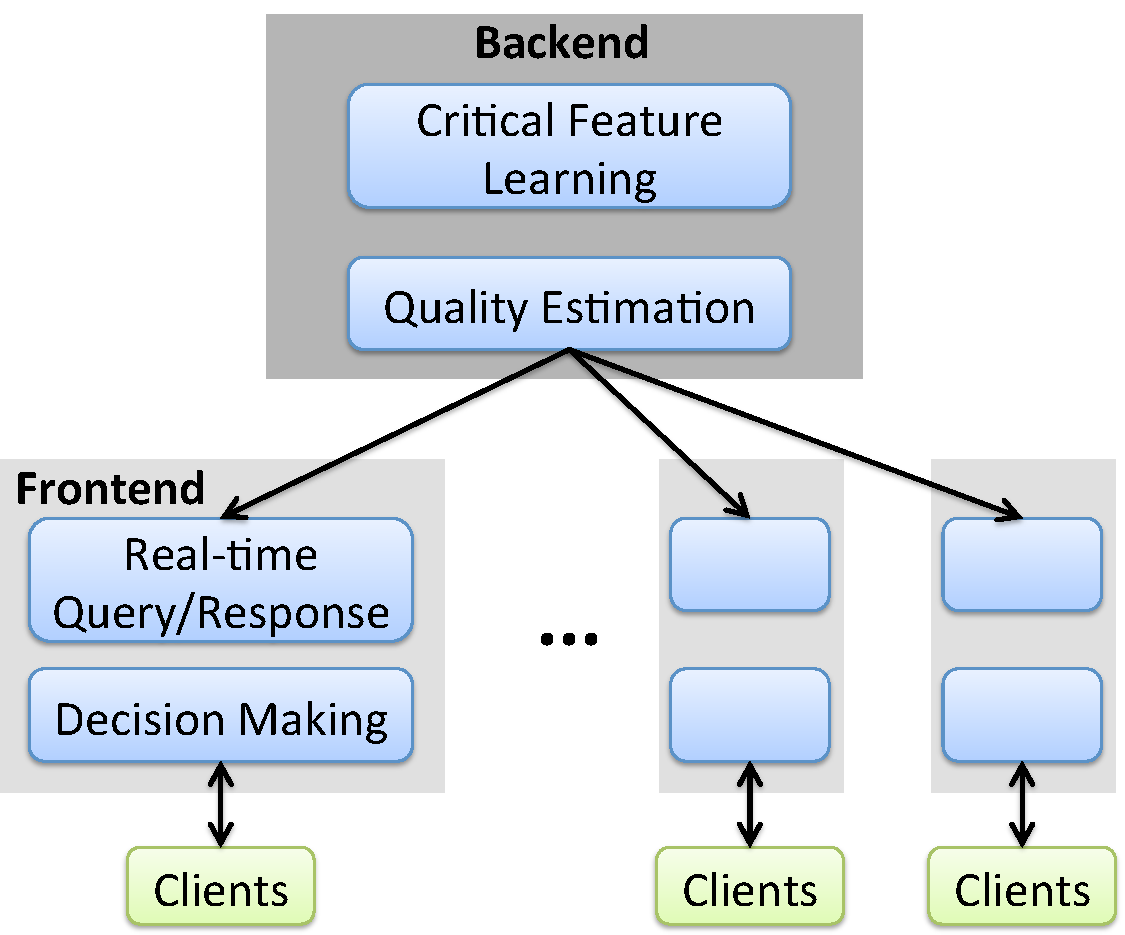
\includegraphics[width=.55\textwidth]{figures/cfa-impl-overview.pdf}
\vspace{-0.1cm}
\caption{Implementation overview of \dda. The three stages of 
\dda workflow are implemented in a backend cluster and distribute
frontend clusters.}
%\vspace{-0.2cm}
\label{fig:impl}
\end{figure}

\mypara{Centralized backend} 
The critical feature learning and quality 
estimation stages are implemented in a backend 
cluster as periodic jobs. 
By default, critical feature learning runs every 30 
minutes, and quality estimation runs every minute. 
A centralized backend is a natural choice because 
we need  a global view of all quality measurements.
The quality function, once updated by the estimation 
step, is disseminated to distributed 
frontend clusters using Kafka~\cite{kreps2011kafka}.

%backend cluster is two-fold.
%First, the backend has the access to the database of 
%all quality measurements, which is needed by critical 
%feature learning and quality estimation.
%Second, they are not required to be as much responsive to client 
%requests as real-time query/response. 

%For real-time query/response to use the up-to-date 
%quality function (i.e., a map between a \leaf and 
%quality estimation), 

Note that we can further reduce learning time
 using simple parallelization strategies. 
%(As discussed in \Section\ref{subsec:scalability}, parallelization alone does not provide a scalable workflow).  
Specifically, the critical features of different \leafs 
can be learned independently.
Similarly in Algorithm~\ref{alg:learning}, the 
similarity  of quality distributions can be 
computed in parallel. 
To exploit this data-level parallelism, 
we implement them as Spark jobs~\cite{spark}. 



\mypara{Distributed frontend} 
%Real-time query/response to prediction queries 
%is implemented in distributed frontend clusters, 
%where decision makers  (which selects CDN, 
%bitrate for clients) are located~\cite{c3}.
Real-time query/response and 
decision makers of CDN/bitrate are co-located in 
distributed frontend clusters that are closer to 
clients than the backend.
%Pushing real-time query/response and 
%decision maker to distributed frontend 
Each frontend cluster receives the quality function 
from the backend and caches it locally for fast
prediction.
This reduces the latency of making decisions 
for clients.
 




%The learning of critical feature function and quality 
%functions on different ``\leafs'' is independent. 
%Critical feature learning can simultaneously 
%evaluate the distribution similarity in 
%Algorithm~\ref{alg:learning} of multiple feature 
%combinations in one ``Map'' operation and find the 
%critical feature in one ``Reduce'' operation. 
%To exploit such parallelism, these two stages are 
%implemented as Spark MapReduce jobs~\cite{spark}. 



\subsection{Challenges in an Operational Setting}
\label{subsec:cfa:impl:challenge}

%Next, we highlight some operational experience from the 
%deployment of \dda in a production system.

\mypara{Mitigating impact of bulk data loading} 
%Resources, such as bandwidth and cluster nodes 
%(sender/receivers) between the quality measurement 
%database and 
The backend cluster is shared 
and runs other delay-sensitive 
jobs; e.g.,  analytics queries from production teams. 
 Since the critical feature learning runs periodically 
and loads a large amount of data ($\approx$30 
GB), it creates spikes in the delays of other jobs 
(Figure~\ref{fig:completion-delay}).  
To address this concern, we engineered a simple 
heuristic to evenly spread the data retrieval where  
we load a small piece of data every few minutes. 
As Figure~\ref{fig:completion-delay} shows, this 
reduces the spikes caused by bulk data loading in 
batch mode.
Note that this does not affect critical feature learning.


\begin{figure}[t!]
\centering
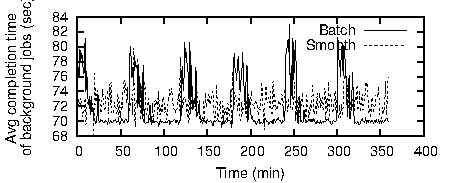
\includegraphics[width=.8\textwidth]{figures/cfa-smooth-batch-timeseries.pdf}
%\vspace{-0.3cm}
\caption{Streaming data loading has smoother 
impact on completion delay than batch data loading.}
%\vspace{-0.4cm}
\label{fig:completion-delay}
\end{figure}

\mypara{Iterative algorithm refinement}
Some parameters (e.g., learning window size 
\HTimeWindowLearn) of \dda require iterative tuning in a 
production environment.
%However, one practical challenge arises  due to code release cycles.
However, one practical challenge is that the 
frontend-facing part of the backend can 
only  be updated once every couple of weeks 
due to code release cycles. 
Thus,  rolling out new prediction algorithms may 
take several days and is a practical concern.
Fortunately, the decoupling between critical feature 
learning and quality estimation 
(Section~\ref{subsec:scalability})
means that changes to critical feature learning
are confined to the backend cluster. 
This enables us to rapidly refine 
and customize the \dda algorithm. 
% (Without this decoupling, any changes to \dda 
%would also need to update quality estimation in the front-end facing part of
%the backend, and would be have slow refresh cycles.)

